\section{Requisitos}
Para representar los requisitos de la aplicación se ha usado UML \cite{uml} por varios
motivos que se expondrán a continuación. El primero de ellos por estar familiarizados
con este, al haber sido usado durante el grado en múltiples ocasiones en asignaturas
distintas. Por otra parte este lenguaje de modelado es un estándar aprobado por la ISO
lo que hace que cualquier diagrama creado pueda ser interpretado de igual forma por
diferentes personas que conozcan el estándar.

\medskip
A continuación se muestran los diagramas UML con los que se han representado los
requisitos de los distintos actores de la aplicación. Solo se ha querido representar los
requisitos que se quieren implementar en esta fase para no cargar con más información de
la necesaria hasta el momento. En el apartado mejoras futuras se nombrarán el resto de ellos.

\medskip
En la figura \ref{casos-de-uso-paciente} se muestran las funcionalidades que el paciente
tiene disponible. Como se puede ver este dispondrá de la posibilidad de ver los ejercicios
y una vez complete estos podrá indicar que se han completado.

\begin{figure}
    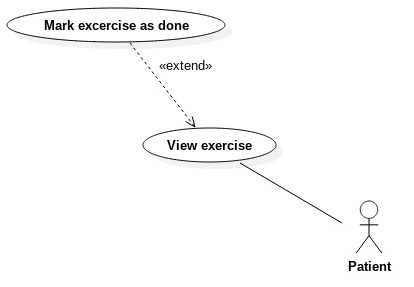
\includegraphics[width=\linewidth]{./images/requisites/use-case-patient.jpeg}
    \caption{Diagrama casos de uso paciente.}
    \label{casos-de-uso-paciente}
\end{figure}

\medskip
Como podemos observar en la figura \ref{casos-de-uso-doctor} el doctor tendrá a su
disposición la posibilidad de realizar una búsqueda entre los pacientes, ver su perfil,
asignar ejercicios y de manera opcional añadirle observaciones a los ejercicios que
asigna. Por último, podrá evaluar la evolución del paciente.

\begin{figure}
    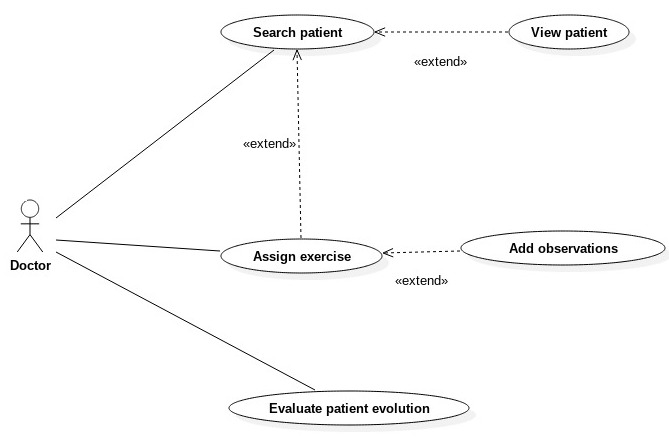
\includegraphics[width=\linewidth]{./images/requisites/use-case-doctor.jpeg}
    \caption{Diagrama casos de uso doctor.}
    \label{casos-de-uso-doctor}
\end{figure}

\medskip
Tal como se muestra en la figura \ref{casos-de-uso-usuarios} de manera genérica todos los
usuarios podrán darse de alta e iniciar sesión en el sistema y ver su propio perfil. Además
de esto, podrán iniciar un chat, enviar mensajes por este, ver los mensajes que se han recibido
y enviar vídeos.

\begin{figure}
    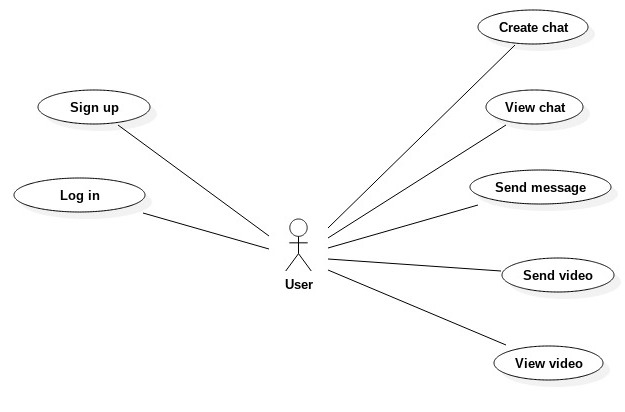
\includegraphics[width=\linewidth]{./images/requisites/use-case-user.jpeg}
    \caption{Diagrama casos de uso usuarios.}
    \label{casos-de-uso-usuarios}
\end{figure}

\medskip
En el siguiente cuadro \ref{tabla-requisitos} se muestran los casos de uso anteriores con una breve descripción.
\begin{table}
    \begin{tabular}{|llp{12cm}|}
        \hline
        ID & ACTOR    & DESCRIPCIÓN \\ \hline
        1  & Usuario  & Puede registrarse en la aplicación \\ \hline
        2  & Usuario  & Puede iniciar sesión en la aplicaicón \\ \hline
        3  & Usuario  & Puede cerrar la sesión \\ \hline
        4  & Usuario  & Puede crear un chat con otra persona \\ \hline
        5  & Usuario  & Puede ver el chat ya creado o que otro usuario ha creado con él \\ \hline
        6  & Usuario  & Puede enviar mensajes por el chat que ha creado u otro usuario
        ha creado co él \\ \hline
        7  & Usuario  & Puede enviar un vídeo en formato mp4 por el chat \\ \hline
        8  & Usuario  & Puede ver el vídeo que le han enviado \\ \hline
        9  & Doctor   & Buscar pacientes en el sistema para asignarle ejercicios o
        consultar su información \\ \hline
        10 & Doctor   & Puede ver el perfil de un paciente que ha buscado \\ \hline
        11 & Doctor   & Puede asignar un ejercicio a un paciente para que este le quede
        reflejadoq que tiene que hacerlo \\ \hline
        12 & Doctor   & En el momento de asignar un ejercicio puede añadir observaciones
        si lo considera el doctor \\ \hline
        13 & Doctor   & Puede consultar la evolución del paciente mirando los ejercicios
        que ha realizado y con que frecuencia \\ \hline
        14 & Paciente & Puede ver el ejercicio que se le ha asignado para consultar las
        observaciones o el ejercicio en sí \\ \hline
        15 & Paciente & Puede marcar como completado un ejercicio que le ha sido asignado \\ \hline
    \end{tabular}

    \caption{Tabla descriptiva de los distintos requisitos.}\label{tabla-requisitos}
\end{table}

% especificacion de casos de uso no la pongo, no hay casos de uso complejos como para explicar

% arquitectura del sistema
%    front
%    back

